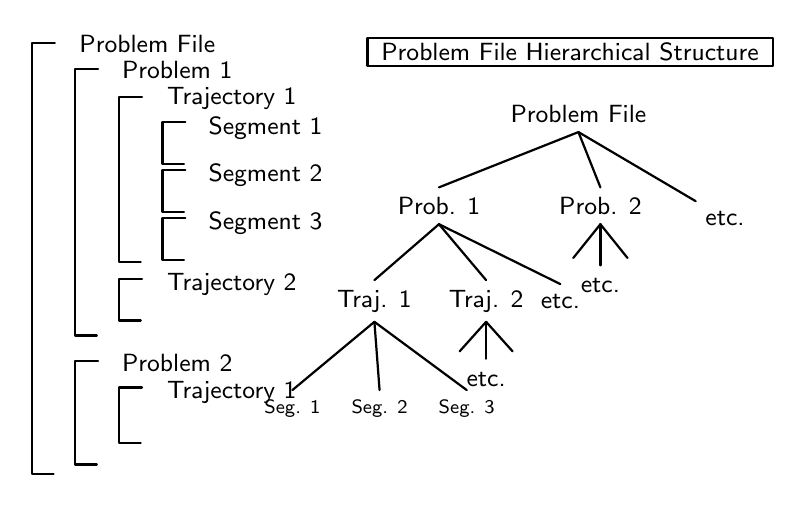
\begin{tikzpicture}[x=0.82cm,y=0.78cm,font=\sffamily\small,line cap=round,line join=round]
  \useasboundingbox (-0.15,0.05) rectangle (11.25,7.45);

  % Left-hand nested-bracket representation from the source figure.
  \draw[line width=0.85pt] (0.25,0.18)--(-0.08,0.18)--(-0.08,7.20)--(0.27,7.20);
  \node[anchor=west] at (0.50,7.18) {Problem File};

  \draw[line width=0.85pt] (0.92,2.44)--(0.58,2.44)--(0.58,6.78)--(0.94,6.78);
  \node[anchor=west] at (1.16,6.76) {Problem 1};

  \draw[line width=0.85pt] (1.60,3.63)--(1.26,3.63)--(1.26,6.32)--(1.62,6.32);
  \node[anchor=west] at (1.86,6.30) {Trajectory 1};

  \draw[line width=0.85pt] (2.27,5.23)--(1.94,5.23)--(1.94,5.91)--(2.29,5.91);
  \draw[line width=0.85pt] (2.27,4.45)--(1.94,4.45)--(1.94,5.13)--(2.29,5.13);
  \draw[line width=0.85pt] (2.27,3.67)--(1.94,3.67)--(1.94,4.35)--(2.29,4.35);
  \node[anchor=west] at (2.50,5.82) {Segment 1};
  \node[anchor=west] at (2.50,5.04) {Segment 2};
  \node[anchor=west] at (2.50,4.26) {Segment 3};

  \draw[line width=0.85pt] (1.60,2.68)--(1.26,2.68)--(1.26,3.36)--(1.62,3.36);
  \node[anchor=west] at (1.86,3.27) {Trajectory 2};

  \draw[line width=0.85pt] (0.92,0.34)--(0.58,0.34)--(0.58,2.02)--(0.94,2.02);
  \node[anchor=west] at (1.16,1.99) {Problem 2};
  \draw[line width=0.85pt] (1.60,0.69)--(1.26,0.69)--(1.26,1.59)--(1.62,1.59);
  \node[anchor=west] at (1.86,1.52) {Trajectory 1};

  % Right-hand tree representation. Nodes are deliberately unboxed to match the
  % historical artwork and branches are separated so labels remain unobstructed.
  \node[draw,line width=0.75pt,inner xsep=5pt,inner ysep=2pt] at (8.25,7.05)
    {Problem File Hierarchical Structure};
  \node (root) at (8.38,6.05) {Problem File};
  \node (p1) at (6.22,4.55) {Prob. 1};
  \node (p2) at (8.72,4.55) {Prob. 2};
  \node (pe) at (10.65,4.35) {etc.};
  \draw[line width=0.8pt] (root.south)--(p1.north);
  \draw[line width=0.8pt] (root.south)--(p2.north);
  \draw[line width=0.8pt] (root.south)--(pe.north west);

  \node (t1) at (5.22,3.00) {Traj. 1};
  \node (t2) at (6.95,3.00) {Traj. 2};
  \node (p1e) at (8.10,3.00) {etc.};
  \draw[line width=0.8pt] (p1.south)--(t1.north);
  \draw[line width=0.8pt] (p1.south)--(t2.north);
  \draw[line width=0.8pt] (p1.south)--(p1e.north);

  \coordinate (p2a) at (8.30,3.70);
  \coordinate (p2b) at (8.72,3.58);
  \coordinate (p2c) at (9.14,3.70);
  \draw[line width=0.8pt] (p2.south)--(p2a);
  \draw[line width=0.8pt] (p2.south)--(p2b);
  \draw[line width=0.8pt] (p2.south)--(p2c);
  \node at (8.72,3.25) {etc.};

  \node[font=\sffamily\scriptsize] (s1) at (3.95,1.25) {Seg. 1};
  \node[font=\sffamily\scriptsize] (s2) at (5.30,1.25) {Seg. 2};
  \node[font=\sffamily\scriptsize] (s3) at (6.65,1.25) {Seg. 3};
  \draw[line width=0.8pt] (t1.south)--(s1.north);
  \draw[line width=0.8pt] (t1.south)--(s2.north);
  \draw[line width=0.8pt] (t1.south)--(s3.north);

  \coordinate (t2a) at (6.54,2.18);
  \coordinate (t2b) at (6.95,2.06);
  \coordinate (t2c) at (7.36,2.18);
  \draw[line width=0.8pt] (t2.south)--(t2a);
  \draw[line width=0.8pt] (t2.south)--(t2b);
  \draw[line width=0.8pt] (t2.south)--(t2c);
  \node at (6.95,1.72) {etc.};
\end{tikzpicture}
